\chapter{Análise do valor agregado}
\label{project-monitoring-report}

A técnica de análise do valor agregado é uma metodologia que combina escopo, cronograma, e medições de recursos para avaliar o desempenho e progresso do projeto.

Os dois principais indicadores da análise de valor agregado são o IDP (índice de desempenho de prazo) e o IDC (índice de desempenho de custo). Estes indicadores podem ser interpretados da seguinte maneira:

\begin{description}
	\item[IDP = 1] Projesto está atendendo as expectativas (dentro do prazo).
	\item[IDP > 1] Projeto está superando as expectativas (adiantado).
	\item[IDP < 1] Projeto está abaixo das expectativas (atrasado).
\end{description}

O gráfico da análise de valor agregado e dos índices de desempenho podem ser vistos na figura \ref{fig:earned-value-analysis}.

\begin{figure}[h]
	\centering
	\begin{tikzpicture}[scale=0.7, every node/.style={scale=0.7}]
		\node at (current page.center) {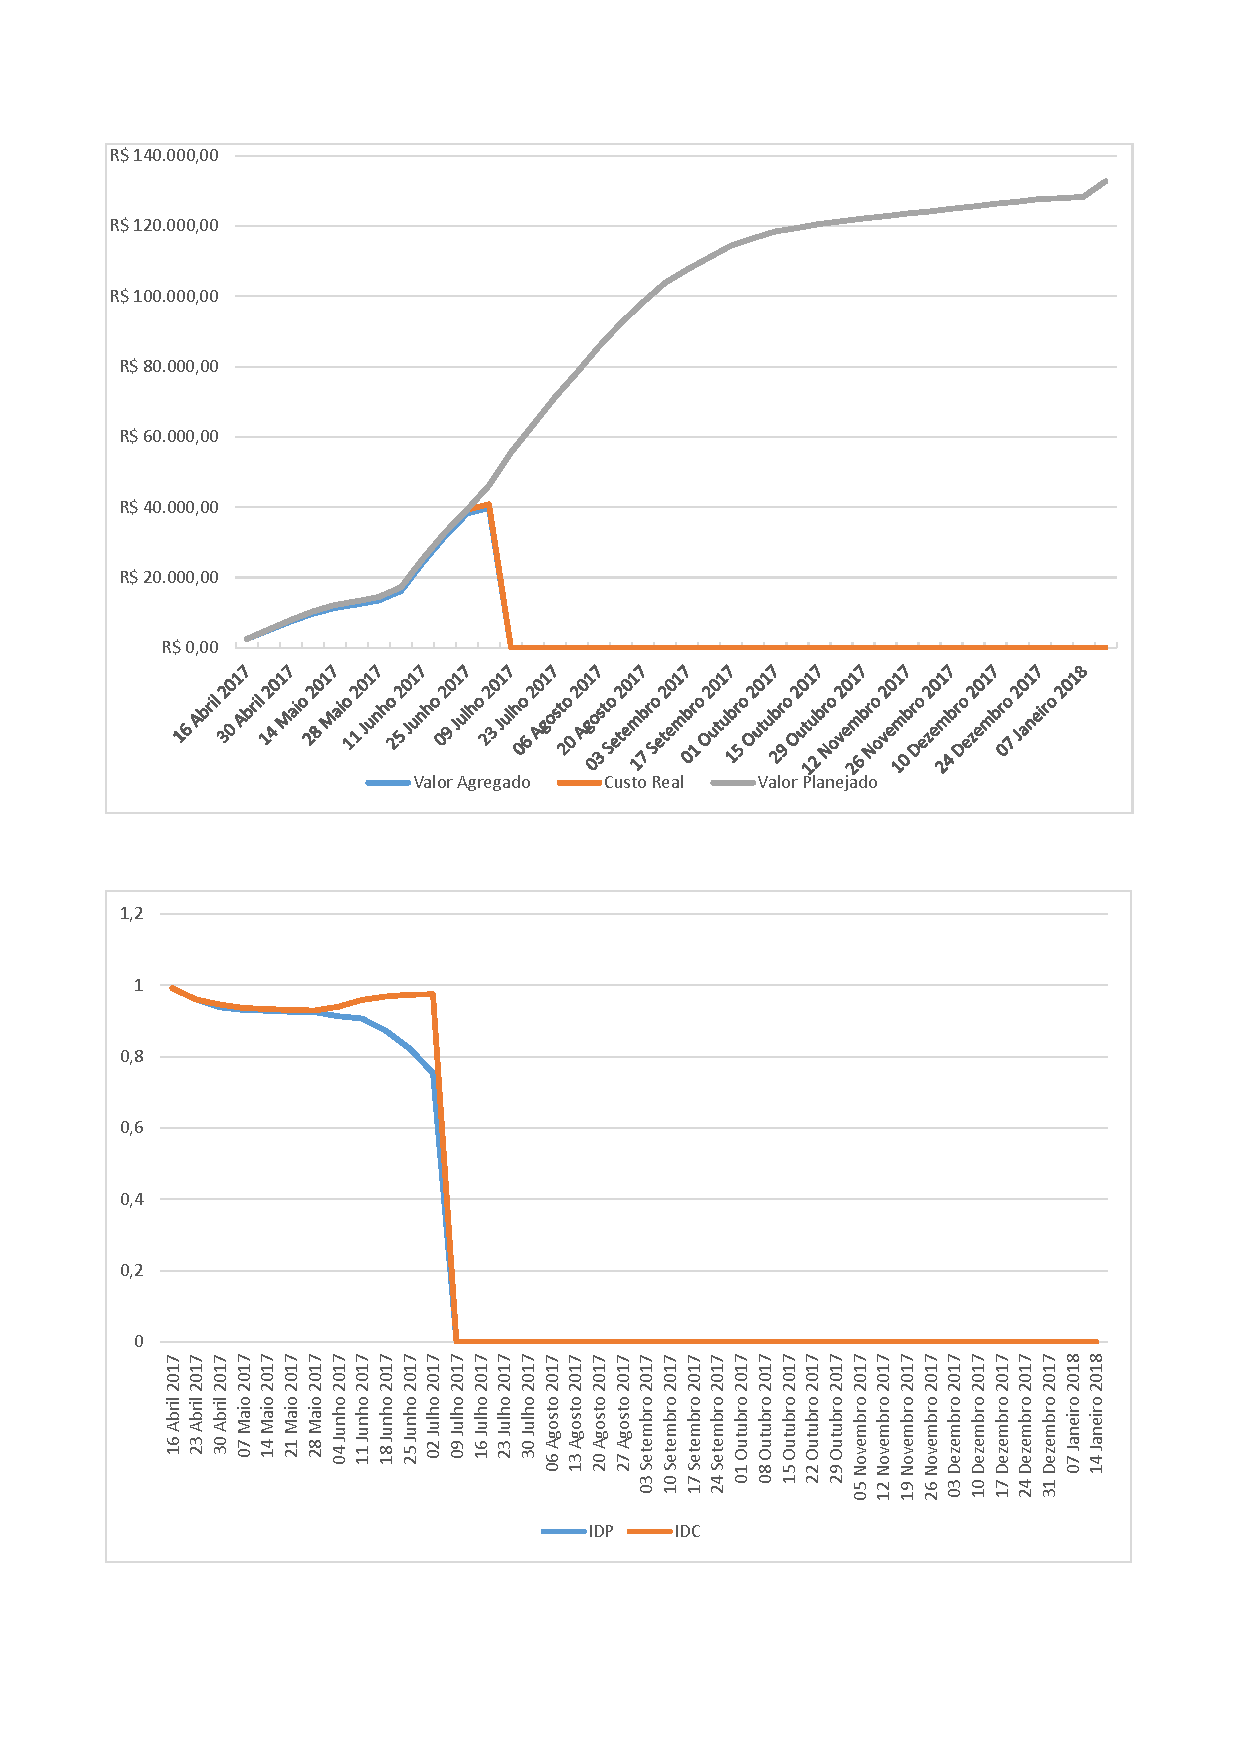
\includegraphics[page=1]{include/earned-value-chart.pdf}};
	\end{tikzpicture}
	\caption{Análise de valor agregado.}
	\label{fig:earned-value-analysis}
\end{figure}